\documentclass[tikz,border=5pt]{standalone}
\usepackage{amsmath,amssymb}
\usetikzlibrary{decorations.pathreplacing,calc,arrows.meta}

\definecolor{accent}{RGB}{0, 100, 170}
\definecolor{highlight}{RGB}{200, 60, 30}
\definecolor{darkgreen}{RGB}{0, 120, 60}
\definecolor{earthblue}{RGB}{40,80,150}
\definecolor{orbitgray}{RGB}{100,100,100}
\definecolor{annulusfill}{RGB}{210,230,250}

\begin{document}
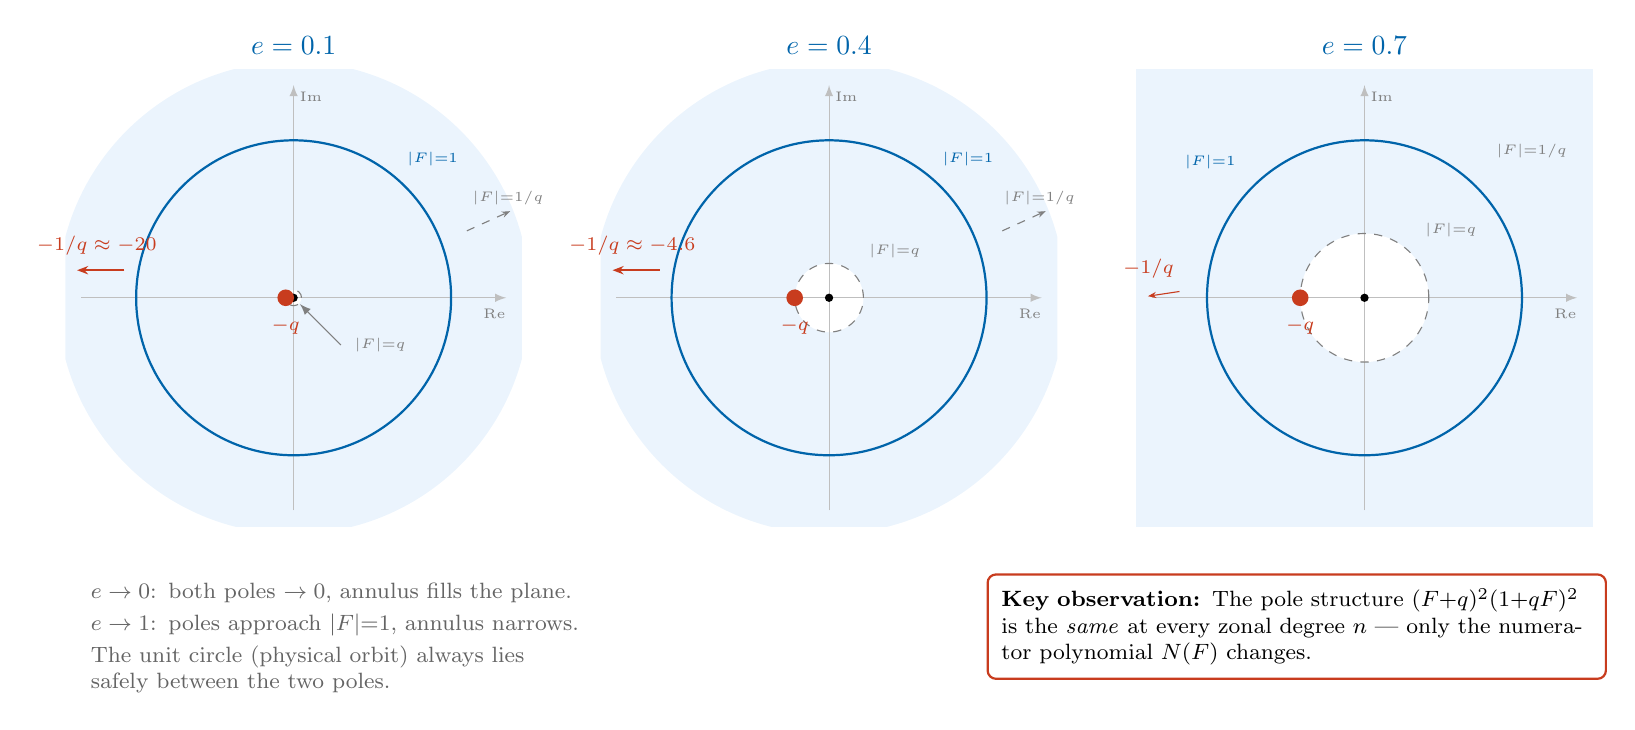
\begin{tikzpicture}[>=latex, font=\small]

% Common scale: unit circle = 2 cm radius
\def\R{2.0}

% ======================================================================
% PANEL 1: e = 0.1,  q = 0.0501,  1/q = 19.97
% ======================================================================
\begin{scope}[shift={(0,0)}]
  \def\qq{0.0501}

  % Panel title (placed outside clip)
  \node[font=\normalsize\bfseries, accent] at (0, \R+1.2) {$e = 0.1$};

  \begin{scope}
    \clip (-2.9, -2.9) rectangle (2.9, 2.9);

    % Annular convergence region
    % Inner radius q*R = 0.10 cm, outer radius 1/q*R ~ 40 cm — fills clip
    \fill[annulusfill, opacity=0.45] (0,0) circle (3.0);
    \fill[white] (0,0) circle ({\qq*\R});

    % Axes
    \draw[gray!50, thin, ->] (-2.7, 0) -- (2.7, 0);
    \draw[gray!50, thin, ->] (0, -2.7) -- (0, 2.7);
    \node[gray, font=\tiny] at (2.55, -0.2) {Re};
    \node[gray, font=\tiny] at (0.22, 2.55) {Im};

    % Inner boundary circle |F| = q (very small, barely visible)
    \draw[gray, dashed, thin] (0,0) circle ({\qq*\R});

    % Unit circle (integration contour)
    \draw[accent, thick] (0,0) circle (\R);

    % Origin
    \fill[black] (0,0) circle (1.5pt);

    % Interior double pole at F = -q (very close to origin)
    \fill[highlight] ({-\qq*\R}, 0) circle (3pt);
  \end{scope}

  % Labels placed outside clip to avoid being cut
  % |F| = 1 label
  \node[accent, font=\tiny] at ({0.707*\R+0.35}, {0.707*\R+0.35}) {$|F|{=}1$};

  % |F| = q label — point to tiny circle
  \draw[gray, thin, ->] (0.6, -0.6) -- (0.08, -0.08);
  \node[gray, font=\tiny, anchor=west] at (0.65, -0.6) {$|F|{=}q$};

  % -q label (below the dot)
  \node[highlight, font=\scriptsize, anchor=north, yshift=-4pt]
    at ({-\qq*\R}, 0) {$-q$};

  % Exterior pole -1/q ~ -20: arrow pointing left with label
  \draw[highlight, thick, -{Stealth[length=4pt]}] (-\R-0.15, 0.35) -- (-2.75, 0.35);
  \node[highlight, font=\scriptsize, anchor=south] at ({-\R-0.5}, 0.42) {$-1/q \approx -20$};

  % 1/q circle indication — arrow pointing out
  \draw[gray, dashed, thin, -{Stealth[length=3pt]}] (\R+0.2, 0.85) -- (2.75, 1.1);
  \node[gray, font=\tiny, anchor=south west] at (\R+0.15, 1.05) {$|F|{=}1/q$};
\end{scope}

% ======================================================================
% PANEL 2: e = 0.4,  q = 0.2182,  1/q = 4.583
% ======================================================================
\begin{scope}[shift={(6.8,0)}]
  \def\qq{0.2182}
  \def\qqinv{4.583}

  % Panel title
  \node[font=\normalsize\bfseries, accent] at (0, \R+1.2) {$e = 0.4$};

  \begin{scope}
    \clip (-2.9, -2.9) rectangle (2.9, 2.9);

    % Annular convergence region
    % outer radius 1/q*R = 9.17 cm — fills clip
    \fill[annulusfill, opacity=0.45] (0,0) circle (3.0);
    \fill[white] (0,0) circle ({\qq*\R});

    % Axes
    \draw[gray!50, thin, ->] (-2.7, 0) -- (2.7, 0);
    \draw[gray!50, thin, ->] (0, -2.7) -- (0, 2.7);
    \node[gray, font=\tiny] at (2.55, -0.2) {Re};
    \node[gray, font=\tiny] at (0.22, 2.55) {Im};

    % Inner boundary circle |F| = q
    \draw[gray, dashed, thin] (0,0) circle ({\qq*\R});

    % Unit circle
    \draw[accent, thick] (0,0) circle (\R);

    % Origin
    \fill[black] (0,0) circle (1.5pt);

    % Interior double pole at F = -q
    \fill[highlight] ({-\qq*\R}, 0) circle (3pt);
  \end{scope}

  % Labels outside clip
  \node[accent, font=\tiny] at ({0.707*\R+0.35}, {0.707*\R+0.35}) {$|F|{=}1$};

  % |F| = q label
  \node[gray, font=\tiny, anchor=south west] at ({0.65*\qq*\R+0.1}, {0.65*\qq*\R+0.1}) {$|F|{=}q$};

  % -q label
  \node[highlight, font=\scriptsize, anchor=north, yshift=-4pt]
    at ({-\qq*\R}, 0) {$-q$};

  % Exterior pole -1/q ~ -4.6: arrow pointing left
  \draw[highlight, thick, -{Stealth[length=4pt]}] (-\R-0.15, 0.35) -- (-2.75, 0.35);
  \node[highlight, font=\scriptsize, anchor=south] at ({-\R-0.5}, 0.42) {$-1/q \approx -4.6$};

  % 1/q circle indication
  \draw[gray, dashed, thin, -{Stealth[length=3pt]}] (\R+0.2, 0.85) -- (2.75, 1.1);
  \node[gray, font=\tiny, anchor=south west] at (\R+0.1, 1.05) {$|F|{=}1/q$};
\end{scope}

% ======================================================================
% PANEL 3: e = 0.7,  q = 0.4082,  1/q = 2.45
% ======================================================================
\begin{scope}[shift={(13.6,0)}]
  \def\qq{0.4082}
  \def\qqinv{2.45}

  % Panel title
  \node[font=\normalsize\bfseries, accent] at (0, \R+1.2) {$e = 0.7$};

  \begin{scope}
    \clip (-2.9, -2.9) rectangle (2.9, 2.9);

    % Annular convergence region — outer circle now visible: radius 2.45*2 = 4.9 cm
    \fill[annulusfill, opacity=0.45] (0,0) circle ({\qqinv*\R});
    \fill[white] (0,0) circle ({\qq*\R});

    % Axes
    \draw[gray!50, thin, ->] (-2.7, 0) -- (2.7, 0);
    \draw[gray!50, thin, ->] (0, -2.7) -- (0, 2.7);
    \node[gray, font=\tiny] at (2.55, -0.2) {Re};
    \node[gray, font=\tiny] at (0.22, 2.55) {Im};

    % Inner boundary circle |F| = q (radius = 0.82 cm, well visible)
    \draw[gray, dashed, thin] (0,0) circle ({\qq*\R});

    % Outer boundary circle |F| = 1/q (radius = 4.9 cm, partially visible)
    \draw[gray, dashed, thin] (0,0) circle ({\qqinv*\R});

    % Unit circle
    \draw[accent, thick] (0,0) circle (\R);

    % Origin
    \fill[black] (0,0) circle (1.5pt);

    % Interior double pole at F = -q
    \fill[highlight] ({-\qq*\R}, 0) circle (3pt);

    % Exterior double pole at F = -1/q (at -4.9 cm, partially visible)
    \fill[highlight] ({-\qqinv*\R}, 0) circle (3pt);
  \end{scope}

  % Labels outside clip
  % |F| = 1 label — upper left quadrant to avoid collision with 1/q label
  \node[accent, font=\tiny, anchor=south east]
    at ({-0.707*\R-0.1}, {0.707*\R+0.1}) {$|F|{=}1$};

  % |F| = q label — right side
  \node[gray, font=\tiny, anchor=south west]
    at ({0.707*\qq*\R+0.07}, {0.707*\qq*\R+0.07}) {$|F|{=}q$};

  % |F| = 1/q label — below |F|=1 label, near visible dashed arc
  \node[gray, font=\tiny, anchor=south west] at (1.55, 1.65) {$|F|{=}1/q$};

  % -q label
  \node[highlight, font=\scriptsize, anchor=north, yshift=-4pt]
    at ({-\qq*\R}, 0) {$-q$};

  % -1/q label — the dot is at x = -4.9, partially clipped; label inside view
  \node[highlight, font=\scriptsize, anchor=south east]
    at (-2.3, 0.12) {$-1/q$};
  \draw[highlight, thin, -{Stealth[length=3pt]}] (-2.35, 0.08) -- (-2.75, 0.02);
\end{scope}

% ======================================================================
% Bottom annotations (below the panels)
% ======================================================================

% Left annotation
\node[anchor=north west, text width=6.5cm, font=\footnotesize, orbitgray]
  at (-2.7, -3.5) {%
  $e \to 0$: both poles $\to 0$, annulus fills the plane.\\[2pt]
  $e \to 1$: poles approach $|F|{=}1$, annulus narrows.\\[2pt]
  The unit circle (physical orbit) always lies\\
  safely between the two poles.};

% Right annotation — key observation
\node[anchor=north west, draw=highlight, rounded corners=3pt,
  line width=0.8pt, inner sep=5pt,
  text width=7.5cm, font=\footnotesize]
  at (8.8, -3.5) {%
  \textbf{Key observation:} The pole structure
  $(F{+}q)^2(1{+}qF)^2$ is the \emph{same}
  at every zonal degree~$n$ --- only the
  numerator polynomial $N(F)$ changes.};

\end{tikzpicture}
\end{document}
